\documentclass[a4paper,12pt]{article} % тип документа
\usepackage[left=3cm,right=2cm,top=2cm,bottom=3cm,bindingoffset=0cm]{geometry}
\usepackage{indentfirst}
\usepackage{cmap}
\usepackage[T2A]{fontenc}			% кодировка
\usepackage[utf8]{inputenc}			% кодировка исходного текста
\usepackage[english,russian]{babel}	% локализация и переносы
\usepackage{amsmath,amsfonts,amssymb,amsthm,mathtools,array} 
\usepackage{wasysym}
\usepackage[labelsep=period]{caption}
\usepackage{graphicx}
\usepackage{pgfplots}
\usepackage{makeidx}
\usepackage{tikz}
\usepackage{pgfplots}
\usepackage{pdfpages}
\usepackage[nottoc,numbib]{tocbibind}
\pgfplotsset{compat=1.18}

\author{Кузнецов Игорь}
\title{}
\date{\today}

\renewcommand{\bottomfraction}{1.0} % часть страницы, которую может занимать графика снизу страницы

\newcolumntype{L}{>{$}l<{$}} % math-mode version of "l" column type
\newcommand{\ZE}{\bar{E}}
\newcommand{\BE}{\partial E}
\newcommand{\CE}{\complement E}
\newcommand{\IE}{\stackrel{\circ}{E}}
\newcommand{\Def}{\textbf{Определение }}
\newcommand{\Ter}{\textbf{Теорема }}
\newcommand{\Utv}{\textbf{Утверждение }}
\newcommand{\Prd}{\textbf{Предложение }}
\newcommand{\Dvo}{\textbf{Доказательство }}
\newcommand{\Imp}{\textbf{(!) }}
\newcommand{\Sld}{\textbf{Следствия: }}
\newcommand{\Svv}[1]{\textbf{Свойства #1:} }
\DeclareMathOperator{\Ree}{Re}
\DeclareMathOperator{\Imm}{Im}
\DeclareMathOperator{\res}{res}
\DeclareMathOperator{\cov}{cov\,}
\DeclareMathOperator{\kH}{\text{кН}}
\DeclareMathOperator{\m}{\text{м}}
\DeclareMathOperator{\kHm}{\kH\cdot\m}

\begin{document}
% \maketitle
\newcommand{\brv}[1]{{\left| #1 \right|}}
\newcommand{\brr}[1]{{\left( #1 \right)}}
\newcommand{\brs}[1]{{\left[ #1 \right]}}
\newcommand{\brc}[1]{{\left\{ #1 \right\}}}
\newcommand{\brn}[1]{{\left\lVert #1 \right\rVert}}
\newcommand{\bra}[1]{{\left\langle #1 \right\rangle}}
\newcommand{\brrl}[1]{{\left( #1 \right]}}
            \newcommand{\brrr}[1]{{\left[ #1 \right)}}
\newcommand{\under}[2]{{\underset{#2}{\underbrace{#1}}}}
\newcommand{\strm}[1]{\underset{#1}{\rightarrow}}

\includepdf{Отчет по практике (2).pdf}
\tableofcontents
\newpage

\section{Введение}

В последние годы нейронные сети получили широкое распространение, они широко используются для анализа и генерации изображений и видео, обработки естественных языков (перевод, чат-боты), медицинской диагностике, финансовых прогнозах и так далее.

Одним из перспективных направлений в этой области являются так называемые PINN -- Physics-Informed Neural Networks, физически-инфор\-мированные нейронные сети. Классические нейронные сети используют большую выборку реальных данных, однако в естественно-научных областях, таких как физика, химия, биология и т.д. зачастую может просто не хватать нужного объёма данных для обучения. PINN способны обойти это ограничения, используя в обучении знания законов физики, описываемые дифференциальными уравнениями в частных производных. Это позволяет использовать неполные и зашумленные данные, что делает их полезными в реальных научных задачах. Однако, вычислительная сложность PINN выше, чем у классических нейронных сетей, что требует большого количества вычислительных мощностей. 

Впервые терми PINN был введён в статье \cite{bib:pinn:first}. В ней автор дал формальное определение PINN'ам и рассмотрел решение нескольких задач: уравнение Шрёдингера, Навье-Стокса, Ален-Чана.

В настоящее время PINN широко применяются моделировании, анализе широкого спектра физических явлений:

В статье \cite{bib:voltogr:1} рассматривается задача симуляции циклической вольтометрии, исследователями было рассмотрено несколько случая: одномерная вольтометрия на дисковом электроде с полубесконечными или тонкослойными граничными условиями, двумерная вольтометрия на микрополосковом электроде и наконец вольтаметрия на края квадратного электрода, количественно определяя неравномерное распределение тока вблизи угла электрода. Для моделирования был использован перцептрон использующий от трёх до шести скрытых словёв, и гиперболический тангенс в качестве функции активации. Полученные исследователями данные хорошо согласуются с решениями этих же задач, полученными другими способами.

Так же PINN применяются для: анализа литий-ионных батарей\cite{bib:lbat:1,bib:lbat:2}, для моделирование теплопереноса в системах со сложной геометрией \cite{bib:heat:1,bib:heat:2}, решения уравнения Навье-Стокса для моделаирования турбулентности \cite{bib:navstock:1}, химической кинематике \cite{bib:chemkin:1,bib:chemkin:2}. Для изучения биологических процессов существует разновидность PINN'ов -- BINN (Biologically-informed neural network) \cite{bib:BINN:1}
\newpage

\section{Постановка задачи}

\subsection{Цель работы}

Рассмотреть уже решённую физическую задачу, решить её с помощью PINN и сравнить полученные данные с изначальным решением, оценить целесообразность применения PINN к задаче.

\subsection{Описание задачи}

На вход нейросети подаются пространственно-временные координаты. На выходе хотим получить различные характеристики исследуемого физического процесса.

\newpage

\section{Теоретическое описание PINN}

Пусть система описывается неким системой дифференциальных уравнений
\begin{equation}F_j(\lambda, u) = 0, X\in\Omega, t > 0\end{equation}
и набором граничных условий
\begin{equation}u(t_0, x_0) = u_0\end{equation}
где $x$ -- пространственные координаты, $\Omega$ -- некоторая область в $\mathbb{R}^n$, $t$ -- время, $u(t,x)$ -- искомая функция описывающая интересующие нас свойства системы (скорость, плотность, потенциал и т.п.), $\lambda$ -- вектор параметров. Для того что бы нейросеть могла обучаться на заданных уравнениях включим эти функции в функцию потерь в виде среднеквадратичной ошибки
\begin{equation}
    MSE = MSE_F + MSE_0
\end{equation}
где
\begin{equation}
    MSE_F = \sum_j\frac{1}{N_F}\sum_{i=1}^{N_F} (F_j(u(t^i_f, x^i_f)))^2
\end{equation}
требует соблюдения дифуров, описывающих процесс, здесь $\brc{t^i_f, x^i_f}_{i=1}^{N_F}$ -- точки коллокации для $F_i$ и
\begin{equation}
    MSE_0 = \frac{1}{N_0}\sum_{i=1}^{N_0} ((u(t^i_0, x^i_0)) - u^i_0)^2
\end{equation}
требует соблюдения граничных условий, $\brr{t^i_0, x^i_0, u^i_0}_{i=1}^{N_0}$ -- начальные и граничные условия $u(t,x)$.

\newpage

\section{Эксперементы}

\subsection{Физическое описание задач}

Для примера возьмём систему из \cite{bib:tutor}. Она описывается следующими уравнениями
$$\begin{aligned}
        \vec{j}                                                               & =
        -D \nabla c - \xi z e c \nabla \Phi + c \vec{u}                                      \\
        \partial_{t} c                                                        & =
        -\nabla \cdot\vec{j}                                                                 \\
        \nabla^2 \Phi                                                         & =
        -4 \pi l_\mathrm{B} k_\mathrm{B}T z c                                                \\
        \rho \big( \partial_t \vec{u} + (\vec{u} \cdot \nabla ) \vec{u} \big) & =
        -\nabla p_H + \eta \nabla^{2} \vec{u} - (k_\mathrm{B}T \nabla c + zec \nabla \Phi) \\
        \nabla \cdot \vec{u}                                                  & =
        0
    \end{aligned}$$

Здесь 
\begin{itemize}
    \item $c$ -- концентрация ионных частиц,
    \item $j$ -- поток плотности,
    \item $\vec{v}$ -- адвективная скорость жидкости,
    \item $e$ -- заряд электрона
    \item $z$ -- валентность частиц,
    \item $\Phi$ -- электростатический потенциал,
    \item $\xi$ -- подвижность частиц,
    \item $D$ -- коэффициент диффузии частиц,
    \item $l_B$ -- длина Бьеррума, $l_B = \frac{e^2}{4\pi\varepsilon k_B T}$
    \item $k_B$ -- постоянная Больцмана,
    \item $T$ -- температура,
    \item $\rho$ -- плотность жидкости
    \item $p_H$ -- гидродинамическое давление
\end{itemize}

Первое уравнение в системе описывает поток плотности, второе электростатику, третье гидродинамику с помощью уравнения Навье-Стокса, четвёртое уравнение несжимаемости жидкости.

Рассмотрим систему щелевых пор, состоящую из двух одноимённо заряженных бесконечных пластин. Выпишем для такой системы граничные условия

$$
    \begin{aligned}
        c(t, X_l)       & = 0.01        \\
        c(t, X_r)       & = 0.01        \\
        c(0, X)         & = 0.002       \\
        \vec{v}(t, X_l) & = 0           \\
        \vec{v}(t, X_r) & = 0           \\
        \vec{v}(0, X)   & = 0           \\
        \Phi(t, X_l)    & = -0.05       \\
        \Phi(t, X_r)    & = -0.05       \\
        \Phi(0, X)      & = -0.009x^2+2
    \end{aligned}
$$
здесь $t$ -- время, $X_l$ -- пространственные координаты, соответствующие левой стенке, $X_r$ -- правой, $x$ в формул для $\Phi(0,x)$ соответствует оси, перпендикулярной пластинам.

\subsection{Вычисление с помощью PINN}

Реализовывать нейросеть будем с помощью библиотеки \texttt{tensorflow}. Для вычисления функции будем использовать обычный трёхслойный перцептрон, на вход ему мы будем подавать пространственно временные координаты, на выходе будем получать концентрацию $c$, скорость $v$ и потенциал $\Phi$. Для обучения мы оберём эту нейросеть в PINN, на вход он получает внутреннюю точку, а так же точку с левой границы, правой границы и точку в начальный момент времени, все 4 точки поочерёдно передаются в нейросеть, для результатов внутренней точки дополнительно вычислим производные с помощью \texttt{tf.GradientTape}. Из всех полученных данных составляем уравнения вида $F(t, X)=0$ и передаём в качестве выхода. В качестве оптимизатора воспользуемся adam'ом, в качестве функции потерь $MSE$. Далее мы обучаем PINN выдавать 0 по всем выходам, подавая для каждого входа случайные точки, это будет означать, что все уравнения выполняются и внутренняя нейросеть выдаёт правильные значения.

Рассмотрим в начале двумерный случай. Скрытые слои будут иметь размеры 80 и 40, входной слой 4, один для концентрации, два для скорости и один для потенциала, функция активации $\tanh$ (гиперболический тангенс). Результат работы после 5000000 итераций показан на графике \ref{fig:2dres}

\begin{figure}[h]
    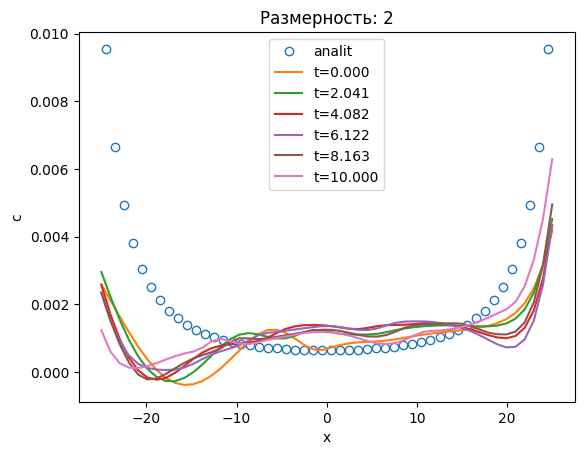
\includegraphics[scale=0.5]{../plots/2dim tanh 80 20.png}
    \caption{}
    \label{fig:2dres}
\end{figure}

Рассмотрим теперь трёхмерный случай. Скрытые слои так же будут иметь размеры 80 и 40, входной слой 5, один для концентрации, три для скорости и один для потенциала, функция активации $relu$. Результат работы после 30000000 итераций показан на графике \ref{fig:3dres}

\begin{figure}[h]
    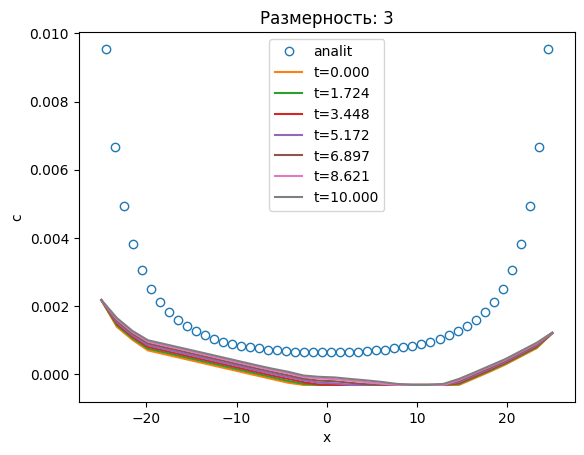
\includegraphics[scale=0.5]{../plots/3dim relu 80 20 30000000.png}
    \caption{}
    \label{fig:3dres}
\end{figure}

\newpage 
\newpage 

\section{Заключение}

Мы написали и протестировали PINN, который решает задачу электрокинетики о системе щелевых пор, состоящих из двух одноимённо заряженных бесконечных пластин. На данном этапе не удалось достичь достаточно точных результатов. Связанно это может быть как со сложностью самих исходных уравнений, так и с недостаточным временем обучения модели. Так же возможно что при задании уравнений была допущена ошибка

\newpage

\bibliographystyle{unsrt}
\bibliography{otchet}

\end{document}